\documentclass[11pt, a4paper, titlepage]{scrartcl}

\usepackage[utf8x]{inputenc}
\usepackage[frenchb]{babel}
\usepackage[T1]{fontenc}
\usepackage{graphicx}
\usepackage{hyperref}
\usepackage{float}

%\renewcommand{\familydefault}{\sfdefault}
%\usepackage[top = 2.54cm, bottom = 2.54cm, left=2.5cm, right=2.5cm]{geometry}

\titlehead{\centering
\includegraphics[width=\textwidth]{images/logo}}
\title{Projet Data Mining}
\author{Pierre \textsc{Turpin}, Jean-Marie \textsc{Comets}}
\date{\today}

\begin{document}

\maketitle
\tableofcontents
\newpage

Au vu des nombreux problèmes de "scaling" que nous pouvions rencontrer
avec le jeu de données prévu, l'intégralité de ce rapport repose sur
l'analyse d'un échantillon de données. Bien entendu, avant d'étudier les
données, nous avons mélangé le jeu de données et pris un échantillon fixe pour
l'ensemble de l'étude.

\section{Caractérisation du flux vidéo}

\subsection{Popularité}

En étudiant les différents indicateurs quantitatifs (attribus *\_count),
représentant le nombre de visionnages d'un flux, nous avons pu remarquer que
quasiment toutes celles-ci sont indépendantes, mis à part l'attribut
\textit{stream\_count}, qui ne représente que la somme du
\textit{embedded\_count} et du \textit{site\_count}. \\

Nous avons donc retiré cet attribut, pour pouvoir définir la notion de
\textbf{popularité} d'un flux, correspondant à une somme normalisée des
différents indicateurs. \\

\subsection{Catégorisation}

Un seul attribut permettant de catégoriser les différents flux est disponible,
et ce uniquement à partir du jeu de données XML : \textit{subcategory}. En
remarquant que cet attribut concerne à la fois la catégorie du jeu et sa
plateforme, nous avons séparé ces deux informations. \\

Ainsi, dans la figure \ref{fig:main_consoles}, nous n'observons pas la
plateforme PC, qui devrait cependant regrouper beaucoup de flux (plateforme non
définie là où le type de jeu est bien défini). Cependant, nous pouvons
remarquer qu'entre les différentes consoles de jeu, c'est la plateforme \textbf{XBOX}
qui a le plus de succès. \\

\begin{figure}[h]
    \centering
    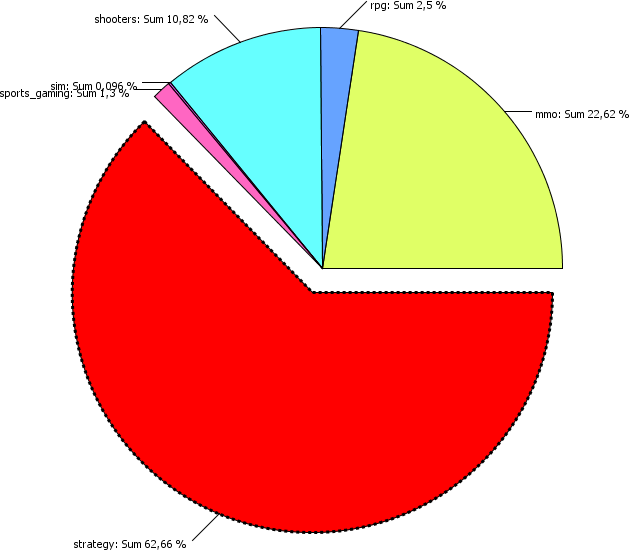
\includegraphics[width=\textwidth]{images/main_categories}
    \caption{Part des vues selon la catégorie du jeu}
    \label{fig:main_categories}
\end{figure}

Nous remarquons à partir de la figure \ref{fig:main_categories} donc que la
catégorie \textbf{strategy} se détache des autres, prenant plus de 60 \% de la
part du nombre de vues des flux. Ceci correspond bien à nos attentes, vu que
Twitch est principalement connu pour des jeux développés pour PC, avec une
préférence pour les jeux de stratégie/roleplay (Starcraft, League of Legends,
etc...).

\begin{figure}[h]
    \centering
    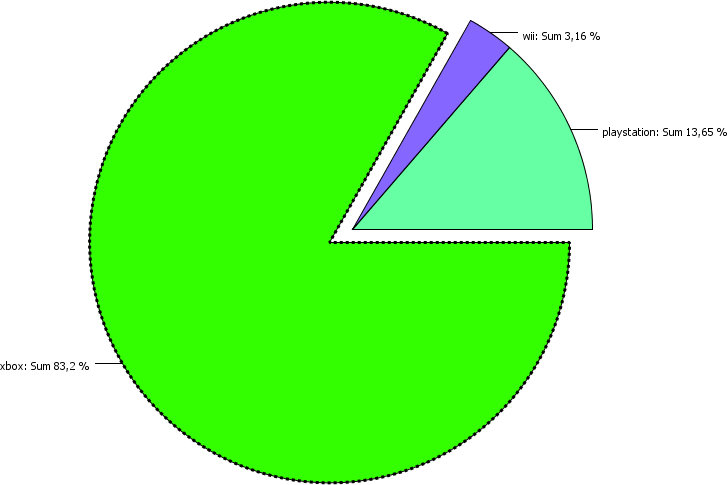
\includegraphics[width=\textwidth]{images/main_consoles}
    \caption{Part des vues selon la plateforme (console) du jeu}
    \label{fig:main_consoles}
\end{figure}

\begin{figure}[h]
    \centering
    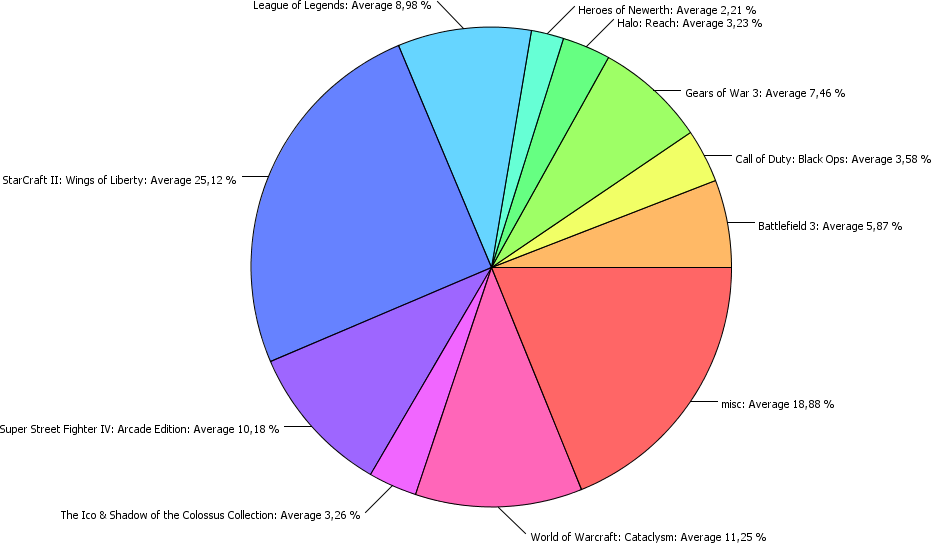
\includegraphics[width=\textwidth]{images/main_games}
    \caption{}
\end{figure}

\begin{figure}[h]
    \centering
    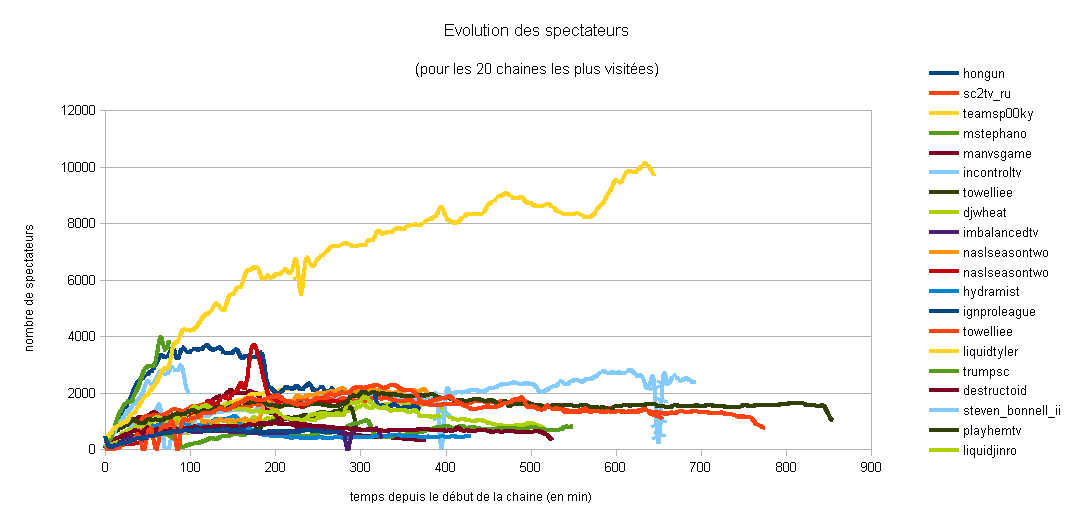
\includegraphics[width=\textwidth]{images/top_20_view_evolutions}
    \caption{}
\end{figure}

\section{Prédiction de l'audience d'un flux}

\begin{figure}[h]
    \centering
    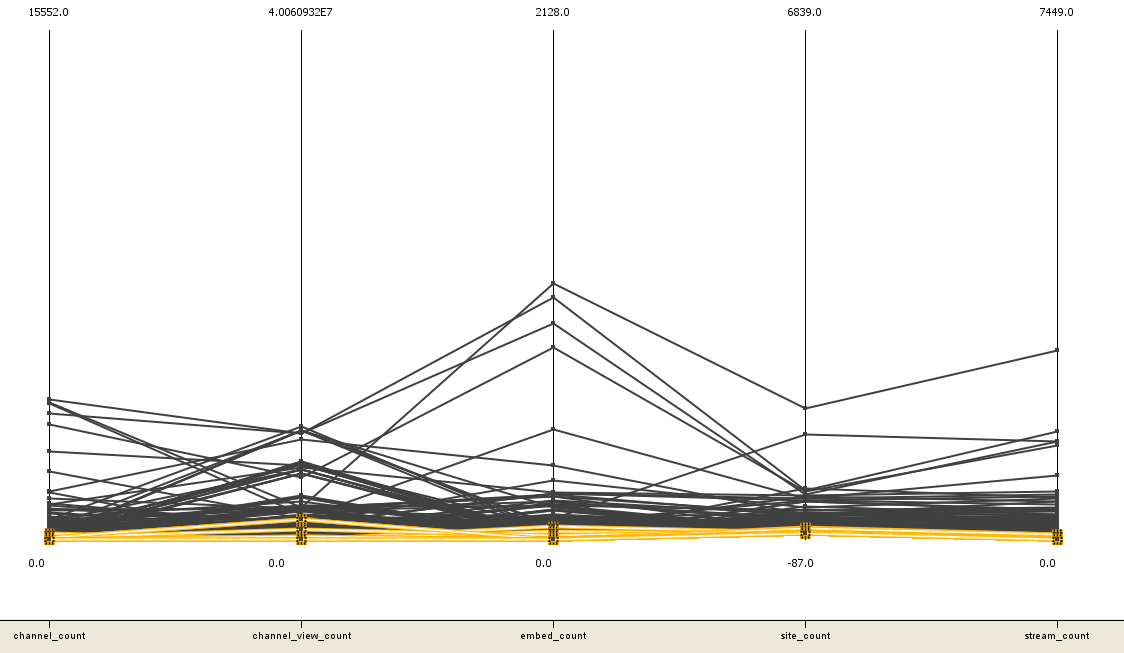
\includegraphics[width=\textwidth]{images/embed_enabled_influence}
    \caption{}
\end{figure}

\begin{figure}[h]
    \centering
    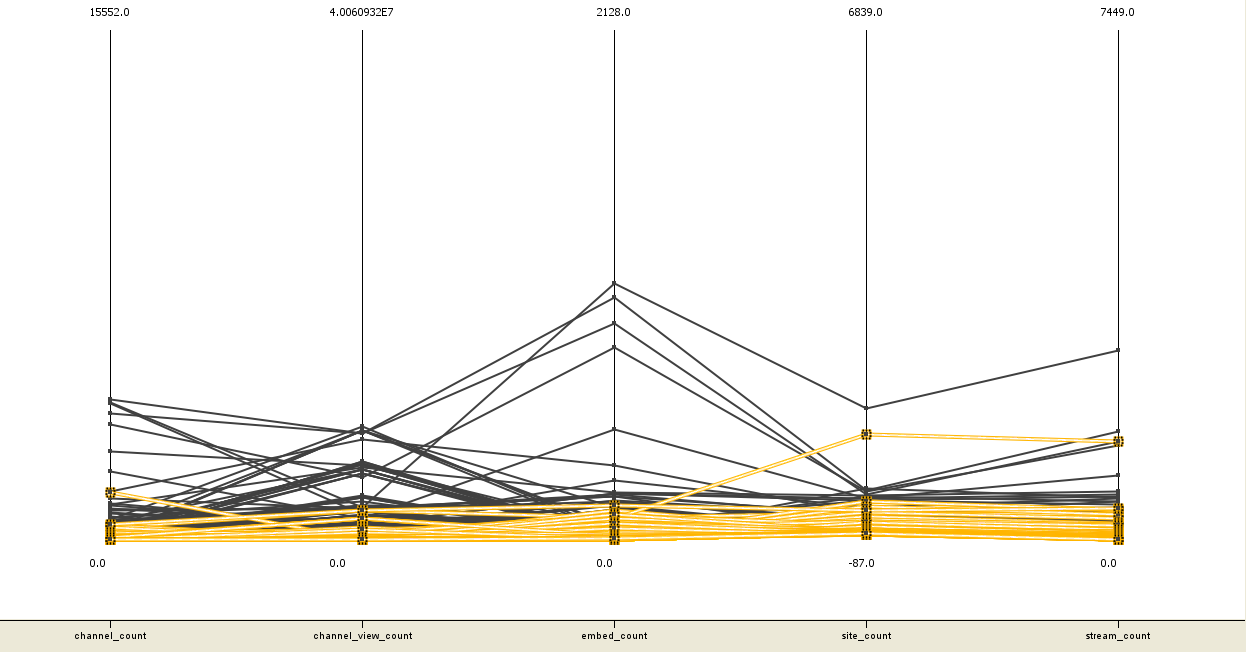
\includegraphics[width=\textwidth]{images/featured_influence}
    \caption{}
\end{figure}

% TODO

\section{Classement des "meilleurs" joueurs}

% TODO classement par tableau/graphe

\end{document}
